
\newpage
\chapter{Interconnect}
{%\hypersetup{linkcolor=black}
\startcontents[chapters]
\printcontents[chapters]{}{1}{}
}

%\noindent\\
%\lipsum[1]

\section{Introduction}
The Vmicro16 processor needs to communicate with multiple peripheral modules (such as UART, timers, GPIO, and more) to provide useful functionality for the end user.

Previous peripheral interface designs of mine have been directly connected to a main driver with unique inputs and outputs that the peripheral required. For example, a timer peripheral would have dedicated wires for it's load and prescaler values, wires for enabling and resetting, and wires for reading. A memory peripheral would have wires for it's address, read and write data, and a write enable signal. This resulted in each peripheral having a unique interface and unique logic for driving the peripheral, which consumed significant amounts of limited FPGA resources.

It can be seen that many of the peripherals need similar inputs and outputs (for example read and write data signals, write enables, and addresses), and because of this, a standard interface can be used to interface with each peripheral. Using a standard interface can reduce logic requirements as each peripheral can be driven by a single driver.

\subsection{Comparison of On-chip Buses}
The choice of on-chip interconnect has changed multiple times over the life-cycle of this project, primary due to ease of implementation and resource requirements. 

Originally, it was planned to use the Wishbone bus \cite{wishbone} due to it's popularity within open-source FPGA modules and good quality documentation.

Late in the project, it was decided to use the AMBA APB protocal \cite {ambaapb}. APB describes an intuitive and easy to implement 2-state interface.

\begin{figure}[H]
\centering
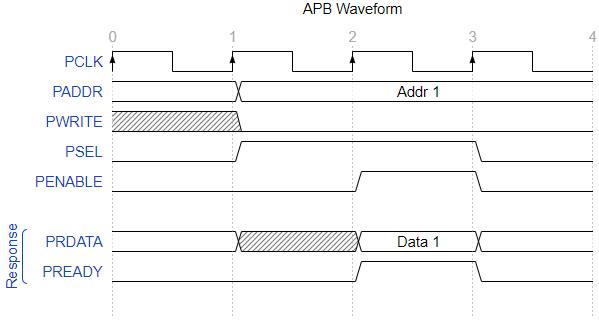
\includegraphics[width=0.7\textwidth]{apb_wave}
\caption{Waveform showing an APB read transaction.}
\end{figure}

\section{Overview}
The system-on-chip design is split into 3 main parts: peripheral interconnect (red), CPU array (gray), and the instruction memory interconnect (green).

A block diagram of this project is shown in Figure \ref{fig:watchdog}
\begin{figure}[H]
\centering
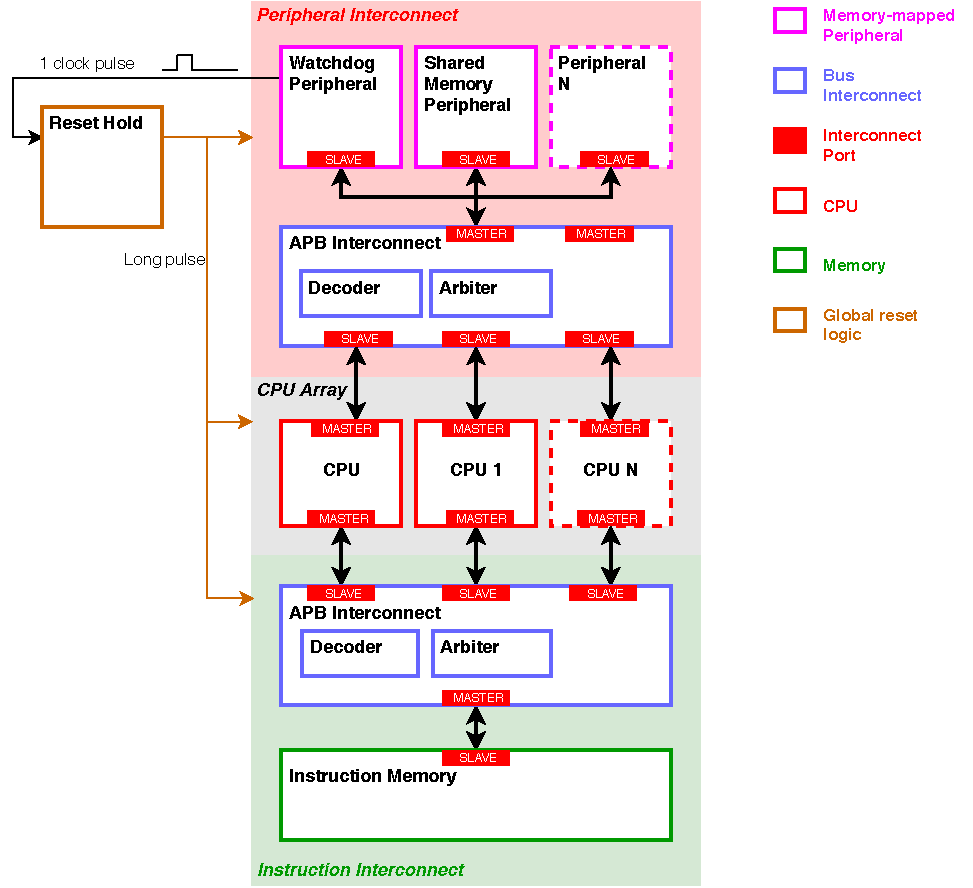
\includegraphics[width=\textwidth]{watchdog}
\caption{Block diagram of the Vmicro16 system-on-chip.}
\label{fig:watchdog}
\end{figure}

\subsection{Design Considerations}
There are several design issues to consider for this project. These are listed below:

\begin{itemize}
\item \textbf{Design size limitations}\\
The target devices for this project are small to medium sized FPGAs (featuring approximately 10,000 to 30,000 logic cells). Because of this, it is important to use a bus interconnect that has a small logic footprint yet is able to scale reasonably well.

\item \textbf{Ease of implementation}\\
The interconnect and any peripherals should be easy to implement within a reasonable time.

\item \textbf{Scalable}\\
The interconnect should allow for easy scalability of master and slave interfaces with minimal code changes.
\end{itemize}

\section{Interfaces}

\begin{figure}[H]
\centering
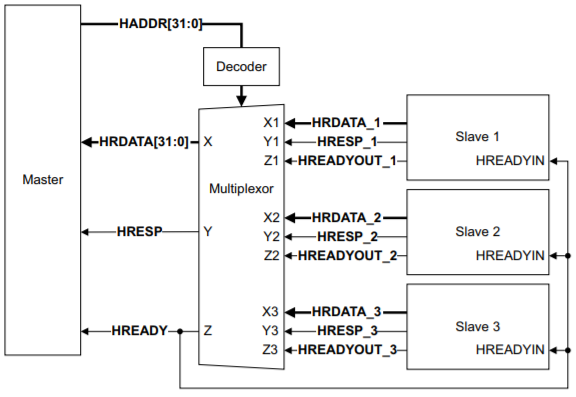
\includegraphics[width=0.7\textwidth]{ahb}
\end{figure}

\subsection{Master to Slave Interface}
\begin{figure}[H]
\centering
\begin{bytefield}[bitwidth=4ex, rightcurly=., rightcurlyspace=0pt]{21}
\bitheader[endianness=big]{0,15,16-20} \\
\begin{rightwordgroup}{PADDR[20:0]}
  \bitbox{1}{\rotatebox{90}{\small LE}}
  \bitbox{1}{\rotatebox{90}{\small SE}}
& \bitbox{3}{\small CORE\_ID}
& \bitbox{16}{Address}
\end{rightwordgroup}\\

\begin{rightwordgroup}{PWDATA[15:0]}
\bitbox{5}{\color{lightgray}\rule{\width}{\height}} & \bitbox{16}{Write data}
\end{rightwordgroup}\\

\begin{rightwordgroup}{PRDATA[15:0]}
\bitbox{5}{\color{lightgray}\rule{\width}{\height}} & \bitbox{16}{Read Data}
\end{rightwordgroup}\\

\begin{rightwordgroup}{PWRITE[0:0]}
\bitbox{20}{\color{lightgray}\rule{\width}{\height}} & \bitbox{1}{\rotatebox{90}{\small WE}}
\end{rightwordgroup}\\

\begin{rightwordgroup}{PENABLE[0:0]}
\bitbox{20}{\color{lightgray}\rule{\width}{\height}} & \bitbox{1}{\rotatebox{90}{\small EN}}
\end{rightwordgroup}
\end{bytefield}
\end{figure}

\newpage
\subsection{Multi-master Support}
\subsubsection{Design Goals}
\begin{enumerate}[leftmargin=3\parindent,label=\bfseries DG\arabic*.]
\item \textbf{Foo}\\
Bing
\end{enumerate}

\begin{figure}[h]
\centering
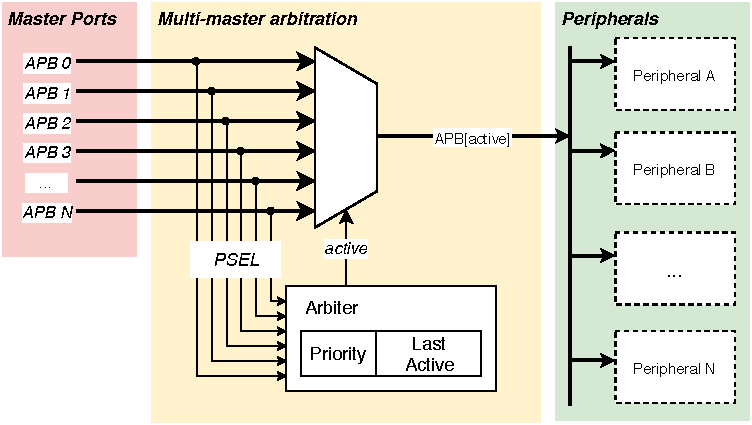
\includegraphics[width=\textwidth]{multimaster}
\caption{Foo}
\label{fig:multimaster}
\end{figure}


\begin{figure}[H]
\centering
\begin{minted}[fontsize=\footnotesize]{verilog}
input      [MASTER_PORTS*BUS_WIDTH-1:0]  S_PADDR,
input      [MASTER_PORTS-1:0]            S_PWRITE,
input      [MASTER_PORTS-1:0]            S_PSELx,
input      [MASTER_PORTS-1:0]            S_PENABLE,
input      [MASTER_PORTS*DATA_WIDTH-1:0] S_PWDATA,
output reg [MASTER_PORTS*DATA_WIDTH-1:0] S_PRDATA,
output reg [MASTER_PORTS-1:0]            S_PREADY,
\end{minted}
\caption{Variable size inputs and outputs to the interconnect.}
\end{figure}

\begin{figure}[H]
\centering
\begin{bytefield}[bitwidth=.5em, rightcurly=., rightcurlyspace=0pt]{84}
\bitheader[endianness=big]{0,20,41,62,83} \\
\bitbox{21}{Core $N$-$1$} & 
\bitbox{21}{$\cdots$} & 
\bitbox{21}{Core 1} & 
\bitbox{21}{Core 0}
\end{bytefield}
\end{figure}


\section{Further Work}
The submitted design is acceptable for a multi-core system as it fulfils the following requirements:
\begin{itemize}
\item Support an arbitrary number of peripherals.
\item Supports memory-mapped address decoding.
\item Supports multiple master interfaces.
\end{itemize}

\chapter{Memory Mapping}
{%\hypersetup{linkcolor=black}
\startcontents[chapters]
\printcontents[chapters]{}{1}{}
}
\noindent\\
The Vmicro16 processor uses a memory-mapping scheme to communicate with peripherals and other cores. This chapter describes the design decisions and implementation of memory-map  used in this project.

\section{Introduction}
Memory mapping is a common technique used by CPUs, micro-controllers, and other system-on-chip devices, that enables peripherals and other devices to be accessed via a memory address on a common bus.

\section{Address Decoding}
An address decoder is used to determine the peripheral that the address is requesting.

After the bus arbiter selects a pending APB interface from the CPU cores, the \verb|PADDR| signal is passed through a decoder module to determine which module the address is asking for.

\begin{figure}[H]
\centering
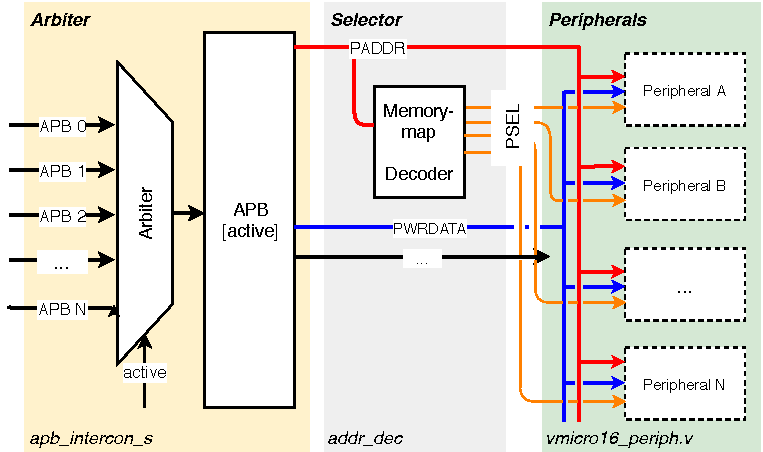
\includegraphics[width=0.8\textwidth]{decoder}
\caption{Foo}
\label{fig:multimaster}
\end{figure}

\subsection{Decoder Optimisations}
In memory-mapped systems, there are two methods used to decode an address bus to perform a chip select (CS). These are full-address and partial-address decoding \cite{tanenbaum2016structured}.

\begin{figure}[H]
\centering
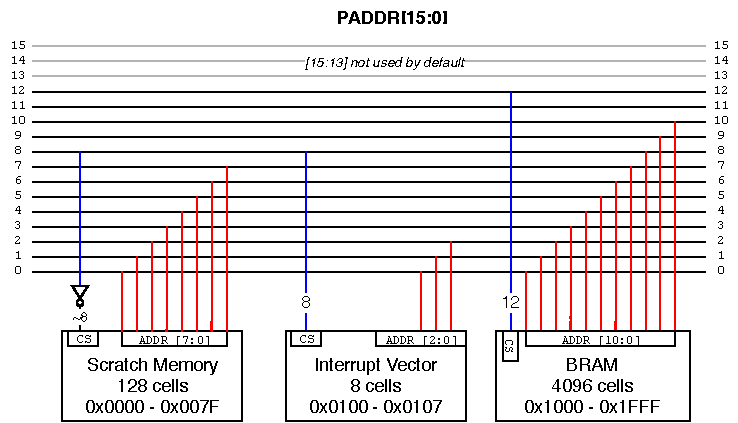
\includegraphics[width=0.8\textwidth]{partial}
\caption{Foo}
\label{fig:multimaster}
\end{figure}

\newpage
\section{Memory Map}
\begin{figure}[H]
\centering
\begin{bytefield}{24}
	\memsection{1FFF}{1000}{8}{Shared Memory with Global Monitor \\ \vspace{.5cm} \tiny See vmicro16\_soc\_config.v}\\
	\bitbox[]{16}{} & \bitbox[]{16}{$\vdots$ \\[1ex]} \\
	
	\begin{rightwordgroup}{Shared peripherals}
	\memsection{0202}{0200}{3}{\nameref{sect:timer}}
	\end{rightwordgroup}\\
	\bitbox[]{16}{} & \bitbox[]{16}{$\vdots$ \\[1ex]} \\
	
	\begin{rightwordgroup}{Per-core instances}
	\memsection{0108}{}{1}{\nameref{sect:interrupts} Mask}\\
	\memsection{0107}{0100}{3}{\nameref{sect:interrupts} Vector}
	\end{rightwordgroup}\\
	
	\bitbox[]{16}{} & \bitbox[]{16}{$\vdots$ \\[1ex]} \\
	
	\begin{rightwordgroup}{Shared peripherals}
	\memsection{00B7}{00B0}{3}{REGS0}\\
	\bitbox[]{16}{} & \bitbox[]{16}{$\vdots$ \\[1ex]} \\
	\memsection{00A1}{00A0}{2}{UART0}\\
	\bitbox[]{16}{} & \bitbox[]{16}{$\vdots$ \\[1ex]} \\
	\memsection{0092}{}{1}{GPIO2}\\
	\memsection{0091}{}{1}{GPIO1}\\
	\memsection{0090}{}{1}{GPIO0}
	\end{rightwordgroup}\\
	\bitbox[]{16}{} & \bitbox[]{16}{$\vdots$ \\[1ex]} \\
	
	\begin{rightwordgroup}{Per-core instances}
	\memsection{008F}{0080}{3}{16 Special Registers}\\
	\memsection{007F}{0000}{8}{Scratch Memory \\ \vspace{.5cm} \tiny See vmicro16\_soc\_config.v}
	\end{rightwordgroup}\\
	
\end{bytefield}
\caption{Memory map showing addresses of various memory sections.}
\label{fig:memmap}
\end{figure}

\newpage
\section{Special Registers}
From the software perspective, it is important for both the developer and software algorithms to know the target system's architecture to better utilise
the resources available to them.
Software written for one architecture with $N$ cores must also run on an architecture with $M$ cores. To enable such portability, the software must query the system for information such as: number of processor cores and the current core identifier. Without this information, the developer would be required to produce software for each individual architecture (e.g. an Intel i5 with 4 cores or an Intel i7 with 8 cores, or an NVIDIA GTX 970 with.

\begin{figure}[H]
\centering
\begin{bytefield}[bitwidth=4ex, rightcurly=., rightcurlyspace=0pt]{16}
\bitheader[endianness=big]{0-15} \\
\begin{rightwordgroup}{0080 R}
\bitbox{8}{\color{lightgray}\rule{\width}{\height}} & \bitbox{8}{CORE\_ID}
\end{rightwordgroup} \\
\begin{rightwordgroup}{0081 R}
\bitbox{8}{\color{lightgray}\rule{\width}{\height}} & \bitbox{8}{NUM\_CORES}
\end{rightwordgroup} \\
\begin{rightwordgroup}{0082 R}
\bitbox{16}{SHARED\_MEMORY cells \tiny(default 4096)}
\end{rightwordgroup} \\
\begin{rightwordgroup}{0083 R}
\bitbox{8}{\color{lightgray}\rule{\width}{\height}} & \bitbox{8}{NUM\_PERIPHERALS}
\end{rightwordgroup} \\
\begin{rightwordgroup}{0084 RW}
\bitbox{16}{User defined}
\end{rightwordgroup} \\
\bitbox[]{16}{$\vdots$ \\[1ex]} \\
\begin{rightwordgroup}{008F RW}
\bitbox{16}{User defined}
\end{rightwordgroup}
\end{bytefield}
\caption{Vmicro16 Special Registers layout (0x0080 - 0x008F).}
\end{figure}


\chapter{Interrupts}
\label{sect:interrupts}
{%\hypersetup{linkcolor=black}
\startcontents[chapters]
\printcontents[chapters]{}{1}{}
}
\noindent\\
This section describes the design, considerations, and implementation, of interrupt functionality within the Vmicro16 processor.

\section{Why Interrupts?}
Interrupts are used to enable asynchronous behaviour within a processor.

Interrupts are commonly used to signal actions from asynchronous sources, for example an input button or from a UART receiver signalling that data has been received.

\section{Hardware Implementation}

\subsection{Context Switching}
When acting upon an incoming interrupt the current state the processor must be saved so that changes from the interrupt handler, such as register writes and branches, do not affect the current state. After the interrupt handler function signals it has finished (by using the \textit{Interrupt Return} \verb|intr| instruction) the saved state is restored.
In the case of the Vmicro16 processor, the program counter \verb|r_pc[15:0]| and register set \verb|regs| instance are the only states that are saved. Going forth, the terms \textit{normal mode} and \textit{interrupt mode} are used to describe what registers the processor should use when executing instructions.

When saving the state, to avoid clocking 128 bits (8 registers of 16 bits) into another register (which would increase timing delays and logic elements), a dedicated register set for the interrupt mode (\verb|regs_isr|) is multiplexed with the normal mode register set (\verb|regs|). Then depending on the mode (identified by the register \verb|regs_use_int|) the processor can easily switch between the two large states without significantly affecting timing.

The timing diagram in Figure \ref{fig:interrupts} visually describes this process.

\begin{figure}[h]
\centering
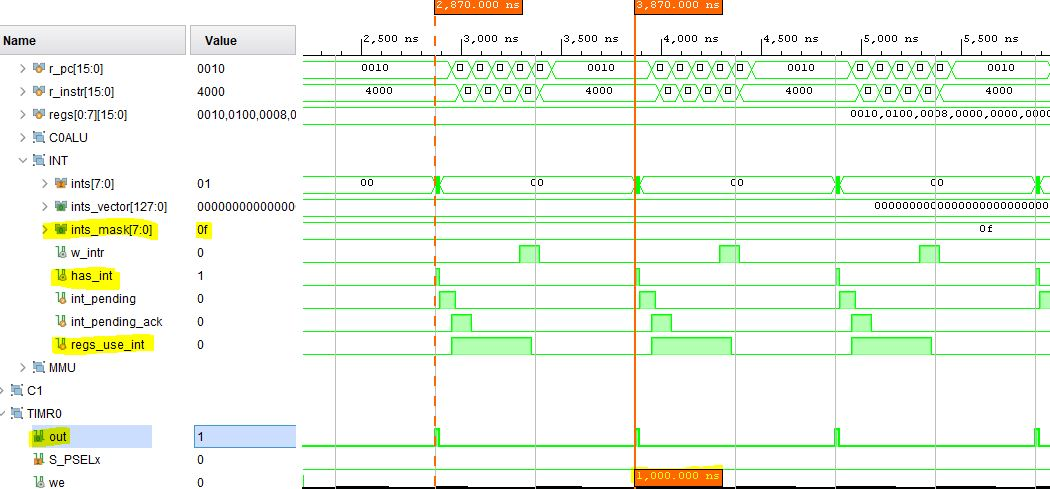
\includegraphics[width=\textwidth]{interrupts}
\caption{Time diagram showing the TIMR0 peripheral emitting a 1us periodic interrupt signal (out) to the processor. The processor acknowledges the interrupt (int\_pending\_ack) and enters the interrupt mode (regs\_use\_int) for a period of time. When the interrupt handler reaches the Interrupt Return instruction (indicated by w\_intr) the processor returns to normal mode and restores the normal state.}
\label{fig:interrupts}
\end{figure}

\section{Software Interface}
To enable software to 

\begin{figure}[H]
\centering
\begin{bytefield}[bitwidth=4ex, rightcurly=., rightcurlyspace=0pt]{16}
\bitheader[endianness=big]{0-15} \\
\begin{rightwordgroup}{0100 RW}
\bitbox{16}{Interrupt handler $0$}
\end{rightwordgroup} \\

\bitbox[]{16}{$\vdots$ \\[1ex]} \\
\begin{rightwordgroup}{0107 RW}
\bitbox{16}{Interrupt handler $7$}
\end{rightwordgroup} \\

\begin{rightwordgroup}{0108 RW}
\bitbox{8}{\color{lightgray}\rule{\width}{\height}} & \bitbox{8}{Interrupt bit mask}
\end{rightwordgroup}
\end{bytefield}
\caption{The interrupt vector consists of eight 16-bit values that point to memory addresses of the instruction memory to jump to.}
\label{fig:r_interrupts}
\end{figure}

\subsection{Interrupt Vector (0x0100-0x0107)}
The interrupt vector is a per-core register that is used to store the addresses of interrupt handlers. An interrupt handler is simply a software function residing in instruction memory that is branched to when a particular interrupt is received. 

\subsection{Interrupt Mask (0x0108)}
The interrupt mask is a per-core register that is used to mask/listen specific interrupt sources. This enables processing cores to individually select which interrupts they respond to. This allows for multi-processor designs where each core can be used for a particular interrupt source, improving the time response to the interrupt for time critical programs. The Interrupt Mask register is an 8-bit read/write register where each bit corresponds to a particular interrupt source and each bit corresponds with the interrupt handler in the interrupt vector.

\begin{figure}
\centering
\begin{bytefield}[bitwidth=4ex]{16}
& \bitlabel{8}{} &
& \bitlabel{6}{[7:2] User defined} &
& \bitlabel{1}{UART0 RX} 
& \bitlabel{1}{TIMR0} \\
\bitheader[endianness=big]{0-7,8,15} \\
  \bitbox{8}{\color{lightgray}\rule{\width}{\height}}
& \bitbox{1}{0}
& \bitbox{1}{0}
& \bitbox{1}{0}
& \bitbox{1}{0}
& \bitbox{1}{0}
& \bitbox{1}{0}
& \bitbox{1}{0}
& \bitbox{1}{0}
\end{bytefield}
\caption{Interrupt Mask register (0x0108). Each bit corresponds to an interrupt source. 1 signifies the interrupt is enabled for/visible to the core. Bits [7:2] are left to the designer to assign.}
\label{fig:r_interruptmask}
\end{figure}

\subsection{Software Example}
To better understand the usage of the described interrupt registers, a simple software program is described below. The following software program produces a simple and power efficient routine to initialise the interrupt vector and interrupt mask.

% pip install pygments-arm
\begin{minted}[fontsize=\footnotesize,linenos,,baselinestretch=0.8]{arm}
entry:
    // Set interrupt vector at 0x100
    // Move address of isr0 function to vector[0]
    movi    r0, isr0
    // create 0x100 value by left shifting 1 8 bits
    movi    r1, #0x1
    movi    r2, #0x8
    lshft   r1, r2
    // write isr0 address to vector[0]
    sw      r0, r1
    
    // enable all interrupts by writing 0x0f to 0x108
    movi    r0, #0x0f
    sw      r0, r1 + #0x8
    halt                  // enter low power idle state
    
isr0:                     // arbitrary name
    movi    r0, #0xff     // do something
    intr                  // return from interrupt
\end{minted}

A more complex example software program utilising interrupts and the TIMR0 interrupt is described in section \ref{sect:timr0_code}.

\section{Design Improvements}
The hardware and software interrupt design have changed throughout the projects cycle. In initial versions of the interrupt implementation, the software program, while waiting for an interrupt, would be in a tight infinite loop (branching to the same instruction). This resulted in the processor using all pipeline stages during this time. The pipeline stages produce many logic transitions and memory fetches which raise power consumption and temperatures. This is quite noticeable especially when running on the Spartan-6 LX9 FPGA.

To improve this, it was decided to implement a new state within the processor's state machine that, when entered, did not produce high frequency logic transitions or memory fetches. The \verb|HALT| instruction was modified to enter this state and the only way to leave is from an interrupt or top-level reset. This removes the need for a software infinite loop that produces high frequency logic transitions (decoding, ALU, register reads, etc.) and memory fetches.

\newpage
\chapter{Peripherals}
{%\hypersetup{linkcolor=black}
\startcontents[chapters]
\printcontents[chapters]{}{1}{}
}

\section{Watchdog Timer}
In any multi-threaded system there exists the possibility for a deadlock -- a state where all threads are in a waiting state -- and algorithm execution is forever blocked.

A common method of detecting a deadlock is to periodically check that a thread is.

\begin{figure}[h]
\centering
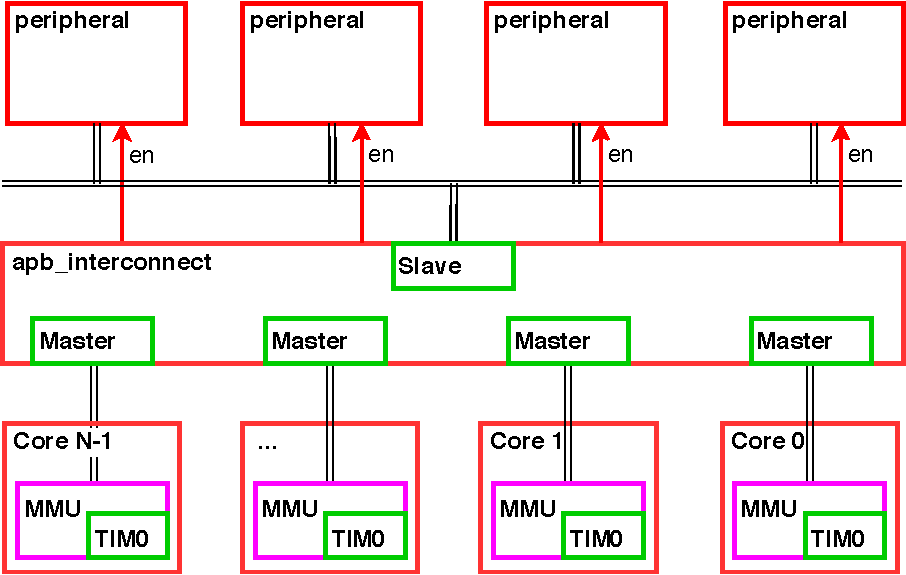
\includegraphics[scale=0.7]{interconnold}
\end{figure}

\section{GPIO Interface}
\begin{figure}[H]
\centering
\begin{bytefield}[bitwidth=4ex, rightcurly=., rightcurlyspace=0pt]{16}
\bitheader[endianness=big]{0-15} \\
\begin{rightwordgroup}{0090 RW}
\bitbox{16}{GPIO0 Output}
\end{rightwordgroup} \\
\begin{rightwordgroup}{0091 RW}
\bitbox{16}{GPIO1 Output}
\end{rightwordgroup} \\
\begin{rightwordgroup}{0092 R}
\bitbox{16}{GPIO1 Input}
\end{rightwordgroup}
\end{bytefield}
\end{figure}


\section{Timer with Interrupt}
\label{sect:timer}
\begin{figure}[H]
\centering
\begin{bytefield}[bitwidth=4ex, rightcurly=., rightcurlyspace=0pt]{16}
\bitheader[endianness=big]{0-15} \\
\begin{rightwordgroup}{0200 RW}
\bitbox{16}{Load Value}
\end{rightwordgroup} \\
\begin{rightwordgroup}{0201 W}
\bitbox{13}{\color{lightgray}\rule{\width}{\height}} &
\bitbox{1}{I} &
\bitbox{1}{R} &
\bitbox{1}{S}
\end{rightwordgroup} \\
\begin{rightwordgroup}{0202 W}
\bitbox{16}{Prescaler}
\end{rightwordgroup}
\end{bytefield}
\end{figure}


\section{UART Interface}
\begin{figure}[H]
\centering
\begin{bytefield}[bitwidth=4ex, rightcurly=., rightcurlyspace=0pt]{16}
\bitheader[endianness=big]{0,1,7,8,15} \\
\begin{rightwordgroup}{00A0 W}
\bitbox{8}{\color{lightgray}\rule{\width}{\height}} & \bitbox{8}{Transmit Data}
\end{rightwordgroup} \\
\begin{rightwordgroup}{00A1 R}
\bitbox{8}{\color{lightgray}\rule{\width}{\height}} & \bitbox{8}{Receive Data}
\end{rightwordgroup} \\
\begin{rightwordgroup}{00A2 R/W}
\bitbox{14}{\color{lightgray}\rule{\width}{\height}} & \bitbox{1}{E} & \bitbox{1}{I}
\end{rightwordgroup}
\end{bytefield}
\end{figure}

\newpage
\chapter{System-on-Chip Layout}
{%\hypersetup{linkcolor=black}
\startcontents[chapters]
\printcontents[chapters]{}{1}{}
}
The Vmicro16 processor uses 

\begin{figure}[H]
\centering
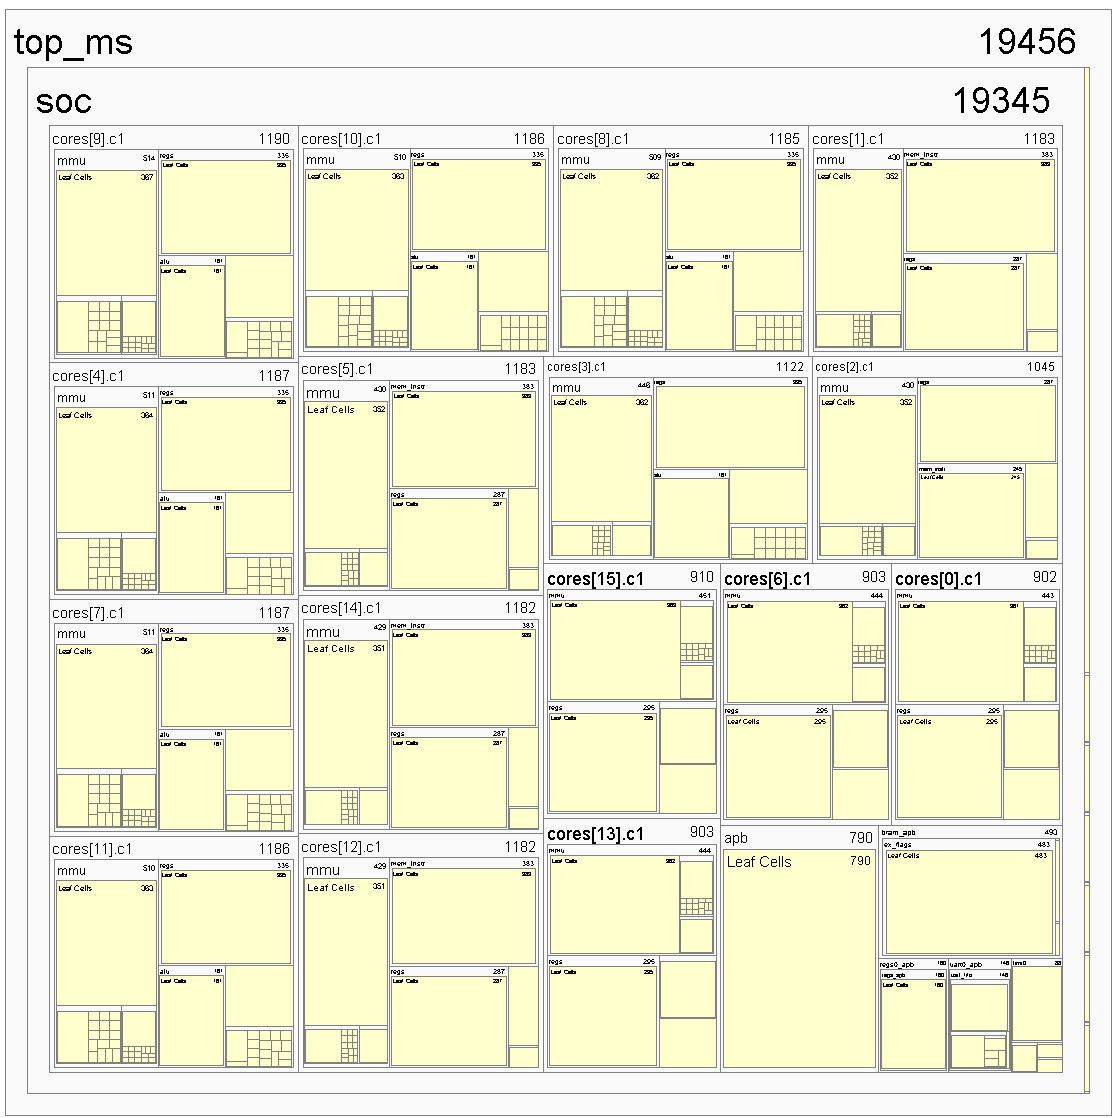
\includegraphics[width=13cm]{soc_layout_schem}
\caption{•}
\label{}
\end{figure}
